\documentclass{article}

% NeurIPS-style workshop paper. [preprint] shows authors (non-anonymous);
% remove the option for a double-blind workshop, or use [final] for camera-ready.
\usepackage[preprint]{neurips_2024}

\usepackage[utf8]{inputenc}
\usepackage[T1]{fontenc}
\usepackage{hyperref}
\usepackage{url}
\usepackage{booktabs}
\usepackage{amsmath,amssymb}
\usepackage{graphicx}
\setcitestyle{numbers,square}  % NeurIPS natbib defaults to author-year; use numeric to match the numbered bibliography below
\graphicspath{{./}}

\title{Audio Spectrogram Transformers Quantize for Free:\\ An Outlier-Free Transformer and a Five-Line INT8-Readiness Diagnostic}

\author{%
  Suleman Imdad \\
  Whiting School of Engineering \\
  Johns Hopkins University, Baltimore, MD, USA \\
  \texttt{suleman361@gmail.com} \\
}

\begin{document}
\maketitle

\begin{abstract}
Vision and language transformers develop \emph{outlier-token activations}: a few tokens whose hidden-state norms grow an order of magnitude larger than the rest. These outliers act as ad-hoc registers and are the dominant failure mode of post-training INT8 quantization, requiring engineering fixes (gated softmax, per-channel scaling, learnable K/V offsets) to recover accuracy. The Audio Spectrogram Transformer (AST) inherits the ViT architecture almost wholesale, so it should inherit both pathologies. We show it does not. Across all twelve encoder layers and 64 ESC-50 clips, AST's patch-token norm distribution is tight and unimodal (final-layer max-to-median ratio $1.23$, outlier rate $0.0\%$). Two consequences follow: register tokens reproduce \emph{mechanically} ($\sim\!8.5\times$ chance attention) but give only a small, non-significant fine-tuning stability gain; and AST tolerates naive post-training INT8 quantization to deployment-grade fidelity (token-state cosine $0.980$--$0.9988$, $49$--$74\%$ smaller) on x86, ARM, and CUDA with no architectural mitigations, unlike BERT and ViT. We propose the max-to-median final-layer norm ratio as a five-line diagnostic for INT8-readiness of any transformer.
\end{abstract}

\section{Introduction}
Two threads in the transformer literature have advanced in parallel. Darcet \emph{et al.}~\cite{darcet2024need} showed that deep transformers develop \emph{outlier-token activations}: a small fraction (1--3\%) of tokens with final-layer norms an order of magnitude larger than typical, concentrated in low-information patches, acting as implicit registers for global information; adding learnable register tokens removes them. Independently, Bondarenko \emph{et al.}~\cite{bondarenko2023quantizable} showed that this same pattern is the dominant failure mode of post-training INT8 (PT-INT8) quantization: outliers force a wide per-tensor dynamic range, starving the bulk of activations of resolution and collapsing accuracy unless mitigations are applied. The two threads describe one phenomenon from opposite angles---an interpretability liability and a deployment liability.

The Audio Spectrogram Transformer (AST)~\cite{gong2021ast} inherits the ViT-Base encoder~\cite{dosovitskiy2021image} almost wholesale---log-mel spectrograms become $16\times16$ patches---yet operates on a modality rich in low-energy ``empty'' regions analogous to the sky and untextured backgrounds where ViT outliers concentrate. If the artifact is a property of the encoder rather than of natural images, AST should exhibit it and be equally quantization-hostile. We find the opposite, and turn that negative result into a deployment win. Our contributions: (1) the first systematic measurement of the Darcet phenomenon in an audio transformer, showing AST is outlier-free across all twelve layers; (2) evidence that the register intervention reproduces mechanically but is \emph{prophylactic rather than corrective} in audio; (3) a demonstration that AST's outlier-free profile makes it uniquely PT-INT8-friendly, plus a norm-ratio diagnostic that predicts INT8-readiness in advance.

\section{Method}
\textbf{Background.} AST embeds spectrogram patches into $d{=}768$-dim tokens, prepends \texttt{[CLS]} and \texttt{[DST]} tokens, and applies $N{=}12$ encoder layers ($H{=}12$ heads). We use the public checkpoint \texttt{MIT/ast-finetuned-audioset-10-10-0.4593} and ESC-50~\cite{piczak2015esc} (2{,}000 clips, 50 classes, 5 folds).

\textbf{Register tokens.} Following~\cite{darcet2024need} we insert $n$ learnable register tokens $\mathbf{r}_1,\ldots,\mathbf{r}_n\sim\mathcal{N}(0,0.02^2)$ between the special tokens and the patch sequence, with no positional embedding; they are visible to all tokens via self-attention but never read by the classifier. At $n{=}4$ this adds $3072$ parameters ($0.004\%$ of AST).

\textbf{Diagnostics.} From the final layer we extract: (a) per-token $\ell_2$ norm $\lVert h_i\rVert_2$ (median, IQR, max), with outlier rate $\Pr[\lVert h_i\rVert_2 > \mathrm{median}+2.5\,\mathrm{IQR}]$; (b) the Frobenius norm $\mathcal{F}_{\text{attn}}$ of the patch--patch sub-block of the head-averaged attention; (c) the fraction of attention mass directed to register columns, against chance $n/(L{+}2{+}n)$.

\textbf{INT8 fidelity and its predictor.} A symmetric per-tensor INT8 quantizer with step $\Delta = x_{\max}/127$ incurs expected per-element error $\Delta/2$. For a median-magnitude element $m$, the relative error is
\begin{equation}
\frac{|\varepsilon_{\text{med}}|}{m}\;\approx\;\frac{x_{\max}}{254\,m}\;=\;\frac{r}{254},
\qquad r \equiv \frac{x_{\max}}{m},
\label{eq:r}
\end{equation}
so the max-to-median ratio $r$ scales bulk quantization error \emph{linearly}. When $r\!\approx\!1$ (AST) the per-element error is $\sim\!0.4\%$; when $r\!\approx\!10$ (ViT-L) it is $\sim\!4\%$, enough to collapse fidelity. We call a model INT8-faithful if token-state cosine to FP32 exceeds $0.99$, top-$5$ prediction-rank agreement exceeds $0.9$, and the $99^{\text{th}}$-percentile relative $\ell_2$ drift is below $0.25$.

\section{Results}
\paragraph{AST is outlier-free.} Table~\ref{tab:diag} reports diagnostics over 64 ESC-50 clips: the patch-norm distribution is tight (median $\approx 32.3$, max $\approx 39.7$), the max-to-median ratio is $1.23$, and the outlier rate is exactly $0.0\%$---versus the order-of-magnitude separation Darcet \emph{et al.} report for ViTs. Fig.~\ref{fig:layerwise} shows this holds at \emph{every} layer (ratio $1.31$--$1.93$, no late-layer phase transition); the early-layer outlier counts in panel (b) reflect a vanishingly small IQR, not high-norm tokens. The artifact simply does not appear in AST.

\paragraph{Registers reproduce but do not repair.} Despite the absence of outliers, register tokens behave exactly as the storage-sink hypothesis predicts (Table~\ref{tab:diag}): register attention mass rises monotonically to $11.2\%$ at $n{=}16$ ($\sim\!8.5\times$ chance), $\mathcal{F}_{\text{attn}}$ falls $\sim\!9\%$, and register tokens immediately occupy a high-norm subspace ($\approx 36$, matching the special tokens). On the canonical ESC-50 5-fold protocol over two seeds (10 fold-runs each), $n{=}4$ registers reduce cross-fold standard deviation from $1.04$ to $0.73$\,pp and lift mean accuracy by $+0.33$\,pp ($92.85\!\to\!93.18\%$); both effects are directionally consistent across seeds but neither is significant ($p{=}0.12$ paired $t$; $p{=}0.15$ one-sided $F$). The intervention is ``no harm, mild positive trend''---registers reorganize attention as designed even with no artifact to remove.

\paragraph{AST is INT8 deployment-friendly.} Because AST lacks the outlier substrate, Eq.~\eqref{eq:r} predicts PT-INT8 should succeed without mitigations. Table~\ref{tab:int8} confirms this on three backends: token-state cosine fidelity $0.980$--$0.9988$, top-5 rank agreement up to $0.95$, size reduction $49$--$74\%$, all from the unmodified checkpoint. The strict cosine-and-rank bar is met cleanly on CUDA; the CPU backends meet the cosine and size bars (top-5 lags under coarse per-tensor dynamic quantization). These numbers exceed PT-INT8 fidelity reported for BERT and ViT~\cite{bondarenko2023quantizable} \emph{without} the gating/clipping those models require. Latency is backend-dependent (only x86+fbgemm is faster, $1.24\times$); the universal, deterministic win is model size and memory---$\sim\!4\times$ multi-tenant GPU density and admission of AST into edge tiers ($86$\,MB vs $329$\,MB) that previously could host only CNNs.

\begin{table}[t]
\caption{Diagnostics on the pretrained AST over 64 ESC-50 clips. Reg.\ mass is attention to register columns (chance in parentheses).}
\label{tab:diag}
\centering\small
\begin{tabular}{cccccc}
\toprule
$n$ & Median & Max & Outlier\% & $\mathcal{F}_{\text{attn}}$ & Reg.\ mass (chance)\\
\midrule
$0$ & $32.26$ & $39.73$ & $0.0$ & $1.820$ & ---\\
$4$ & $32.39$ & $39.64$ & $0.0$ & $1.763$ & $3.9\%$ ($0.33\%$)\\
$16$ & $32.55$ & $39.72$ & $0.0$ & $1.658$ & $11.2\%$ ($1.31\%$)\\
\bottomrule
\end{tabular}
\end{table}

\begin{table}[t]
\caption{PT-INT8 fidelity across three deployment backends (unmodified AST). Baseline is FP32 (CPU) / FP16 (GPU). Right block: cross-study comparison to other families (heterogeneous metrics; illustrative only). ``Fix'' = outlier mitigation required.}
\label{tab:int8}
\centering\small
\begin{tabular}{lccc@{\hskip 1.5em}lccc}
\toprule
Metric & x86 & M1 & A4000 & Family & Max/med & Naive INT8 & Fix?\\
\midrule
Cosine        & $0.980$ & $0.993$ & $\mathbf{0.9988}$ & BERT-B~\cite{bondarenko2023quantizable} & $\sim6$ & $-53$\,pp & gated\\
Top-5 agree.  & $0.730$ & $0.834$ & $\mathbf{0.947}$  & ViT-T~\cite{bondarenko2023quantizable} & $\sim5$ & $-4$\,pp & gated\\
Size reduc.   & $74\%$  & $74\%$  & $49\%$            & LLaMA-7B~\cite{sun2024massive} & $\sim50$ & ppl rise & K/V bias\\
              &         &         &                   & \textbf{AST} & $\mathbf{1.23}$ & \textbf{cos .998} & \textbf{none}\\
\bottomrule
\end{tabular}
\end{table}

\begin{figure}[t]
\centering
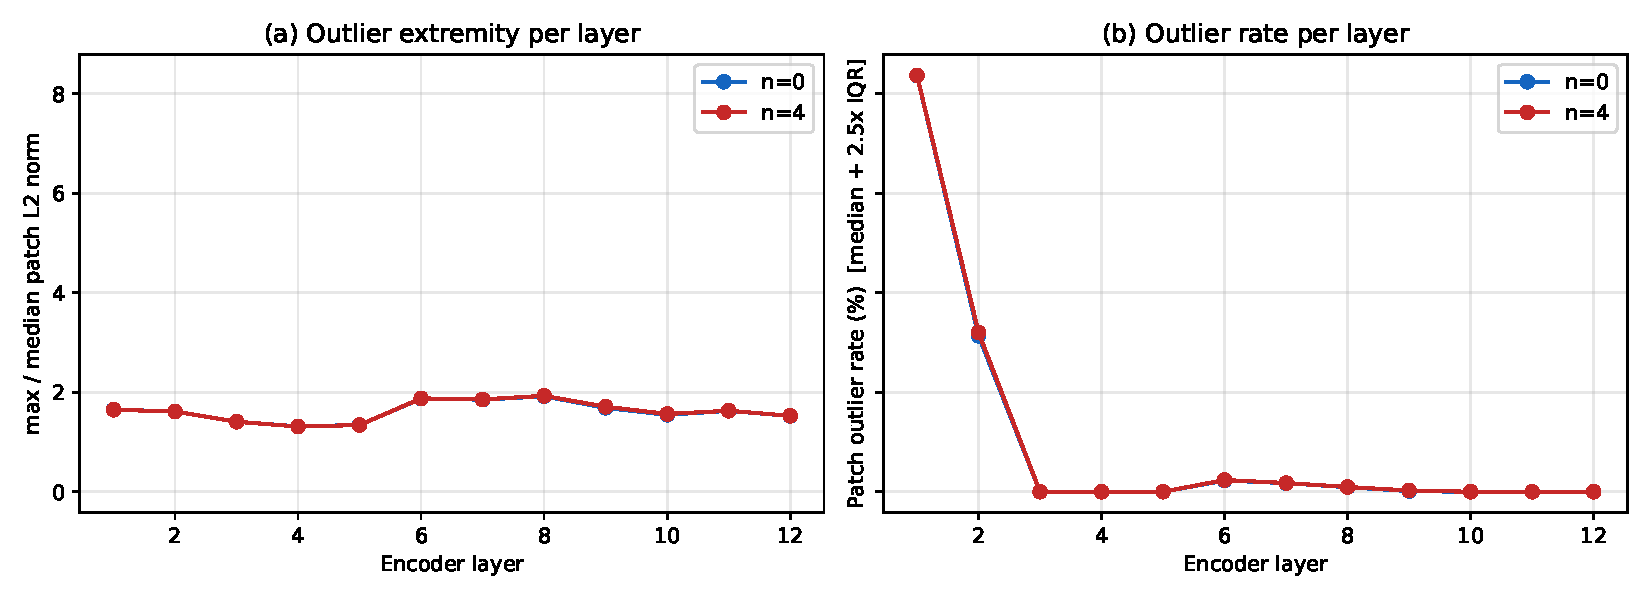
\includegraphics[width=0.82\linewidth]{fig_layerwise_norms.pdf}
\caption{AST is outlier-free at every encoder layer. (a) Max-to-median patch-norm ratio stays in $1.31$--$1.93$. (b) Outlier rate is $0\%$ in the final three layers; early-layer values are an artifact of tiny early-layer IQR (ratio $\leq 1.7$), not Darcet-style high-norm tokens.}
\label{fig:layerwise}
\end{figure}

\begin{figure}[t]
\centering
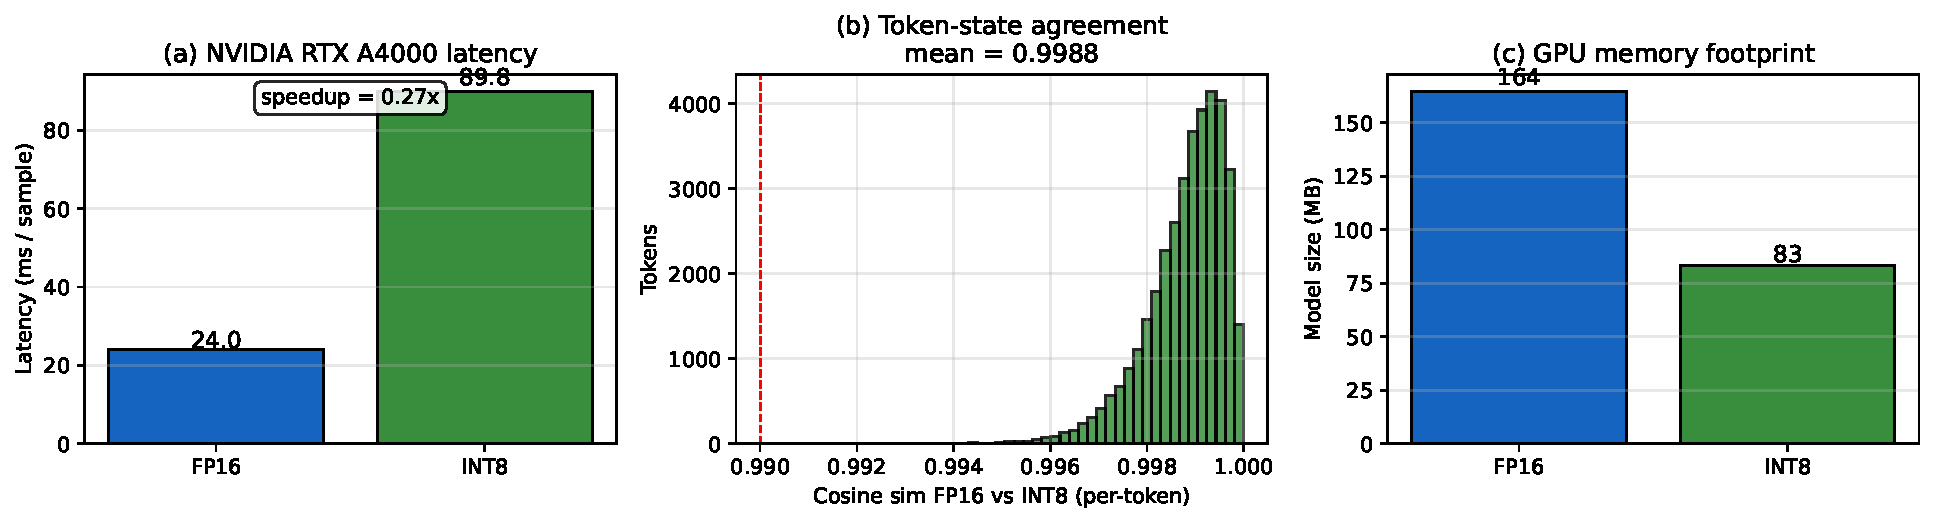
\includegraphics[width=0.62\linewidth]{fig_cuda_quantization.pdf}
\caption{CUDA PT-INT8 (RTX A4000, bitsandbytes): token-state cosine $0.9988$ to FP16 across $30\times1216$ tokens, $49\%$ smaller, no mitigations.}
\label{fig:cuda}
\end{figure}

\section{Why AST Is Outlier-Free, and Conclusion}
The post-Darcet literature converges on conditions for outlier emergence; AST violates several at once~\cite{darcet2024need,sun2024massive,puccetti2022outlier,gu2025emergence}. It is ViT-\emph{Base} scale (Darcet report outliers only in the largest models); it has \emph{no discrete vocabulary}---Puccetti \emph{et al.}~\cite{puccetti2022outlier} explicitly failed to find outliers in audio transformers, attributing this to vocabulary; it is shallow (12 layers) with moderate context, so the over-mixing pressure that drives sink emergence~\cite{gu2025emergence} is weak; and spectrogram ``silence'' still carries non-negligible energy. An architecture identical to ViT on paper does not inherit ViT's pathologies, because those depend on scale, recipe, and modality. For AST this is a gift: registers are a no-regret addition and naive PT-INT8 is a low-risk deployment default. We recommend reporting the max-to-median final-layer norm ratio ($r{<}2$ safe, $r{>}5$ needs a fix) as a five-line INT8-readiness check for any new transformer. Code and data: \url{https://github.com/real1900/silence-in-the-noise}.

\begin{thebibliography}{9}
\bibitem{darcet2024need} T. Darcet, M. Oquab, J. Mairal, and P. Bojanowski. Vision transformers need registers. In \emph{ICLR}, 2024.
\bibitem{bondarenko2023quantizable} Y. Bondarenko, M. Nagel, and T. Blankevoort. Quantizable transformers: removing outliers by helping attention heads do nothing. In \emph{NeurIPS}, 2023.
\bibitem{gong2021ast} Y. Gong, Y.-A. Chung, and J. Glass. AST: Audio spectrogram transformer. In \emph{Interspeech}, 2021.
\bibitem{dosovitskiy2021image} A. Dosovitskiy et al. An image is worth 16x16 words: transformers for image recognition at scale. In \emph{ICLR}, 2021.
\bibitem{piczak2015esc} K. J. Piczak. ESC: dataset for environmental sound classification. In \emph{ACM MM}, 2015.
\bibitem{sun2024massive} M. Sun, X. Chen, J. Z. Kolter, and Z. Liu. Massive activations in large language models. In \emph{COLM}, 2024.
\bibitem{puccetti2022outlier} G. Puccetti, A. Rogers, A. Drozd, and F. Dell'Orletta. Outlier dimensions that disrupt transformers are driven by frequency. In \emph{Findings of EMNLP}, 2022.
\bibitem{gu2025emergence} X. Gu et al. When attention sink emerges in language models: an empirical view. In \emph{ICLR}, 2025.
\end{thebibliography}

\end{document}
